\subsection{Benchmark Overview}
\label{sec:benchmark_overview}

Existing semantic occupancy benchmarks~\cite{OpenOccupancy,Occ3D} are mostly
ego-centric, with labels defined around a moving ego vehicle and a viewpoint that
changes over time; under a fixed roadside viewpoint, by contrast, persistent
static layout and sparse, transient dynamic participants coexist in the same
dense representation, yielding a different problem structure
(Sec.~\ref{sec:introduction}). As summarized in
Table~\ref{tab:dataset_comparison}, existing real-world datasets are either
ego-centric occupancy or object-level roadside/cooperative detection, and none
provides dense semantic occupancy under real fixed roadside sensing.

To fill this gap, we introduce InfraOcc, which constructs dense voxel-level
semantic occupancy annotations in a fixed roadside coordinate system, supports
unified camera-only, LiDAR-only, and multi-modal evaluation, and provides
diagnostic metrics that separate static and dynamic occupancy. Its design goal is
to make the static--dynamic asymmetry of roadside scenes \emph{constructible},
\emph{measurable}, and \emph{evaluable}: a static--dynamic decoupled annotation
pipeline makes it constructible, temporal and semantic diagnostics make it
measurable, and a static/dynamic evaluation protocol makes it evaluable.

\subsection{Infrastructure-side Occupancy Task}
\label{sec:benchmark_task}

Unlike vehicle-centric occupancy perception, InfraOcc defines the occupancy
field in a fixed roadside coordinate system that remains invariant over time and
is shared by all frames in the same scenes. The infrastructure-side occupancy task is
formulated as learning a mapping
\begin{equation}
  \mathcal{F}_{\theta}:\ \mathcal{O}_t \;\longmapsto\;
  \mathbf{Y}_t \in (\mathcal{C}\cup\{\mathrm{free}\})^{X\times Y\times Z},
\end{equation}
where the observation
$\mathcal{O}_t\in\{\mathcal{I}_t,\mathcal{P}_t,(\mathcal{I}_t,\mathcal{P}_t)\}$
corresponds to the roadside sensor measurements at timestamp $t$, consisting of
multi-view images $\mathcal{I}_t$, infrastructure-side LiDAR point clouds
$\mathcal{P}_t$, or their combination. The prediction
$\mathbf{Y}_t$ represents a dense semantic occupancy volume over the shared
roadside voxel space, where each voxel is assigned either a semantic occupancy
label from $\mathcal{C}$ (e.g., vehicle, pedestrian, vegetation, or road
surface) or the free-space label. To facilitate consistent evaluation, the
camera-only ($\mathcal{I}_t$), LiDAR-only ($\mathcal{P}_t$), and multi-modal
($(\mathcal{I}_t,\mathcal{P}_t)$) tracks adopt the same voxelization scheme,
semantic label set, and evaluation protocol.
\begin{figure}[t]
  \centering
  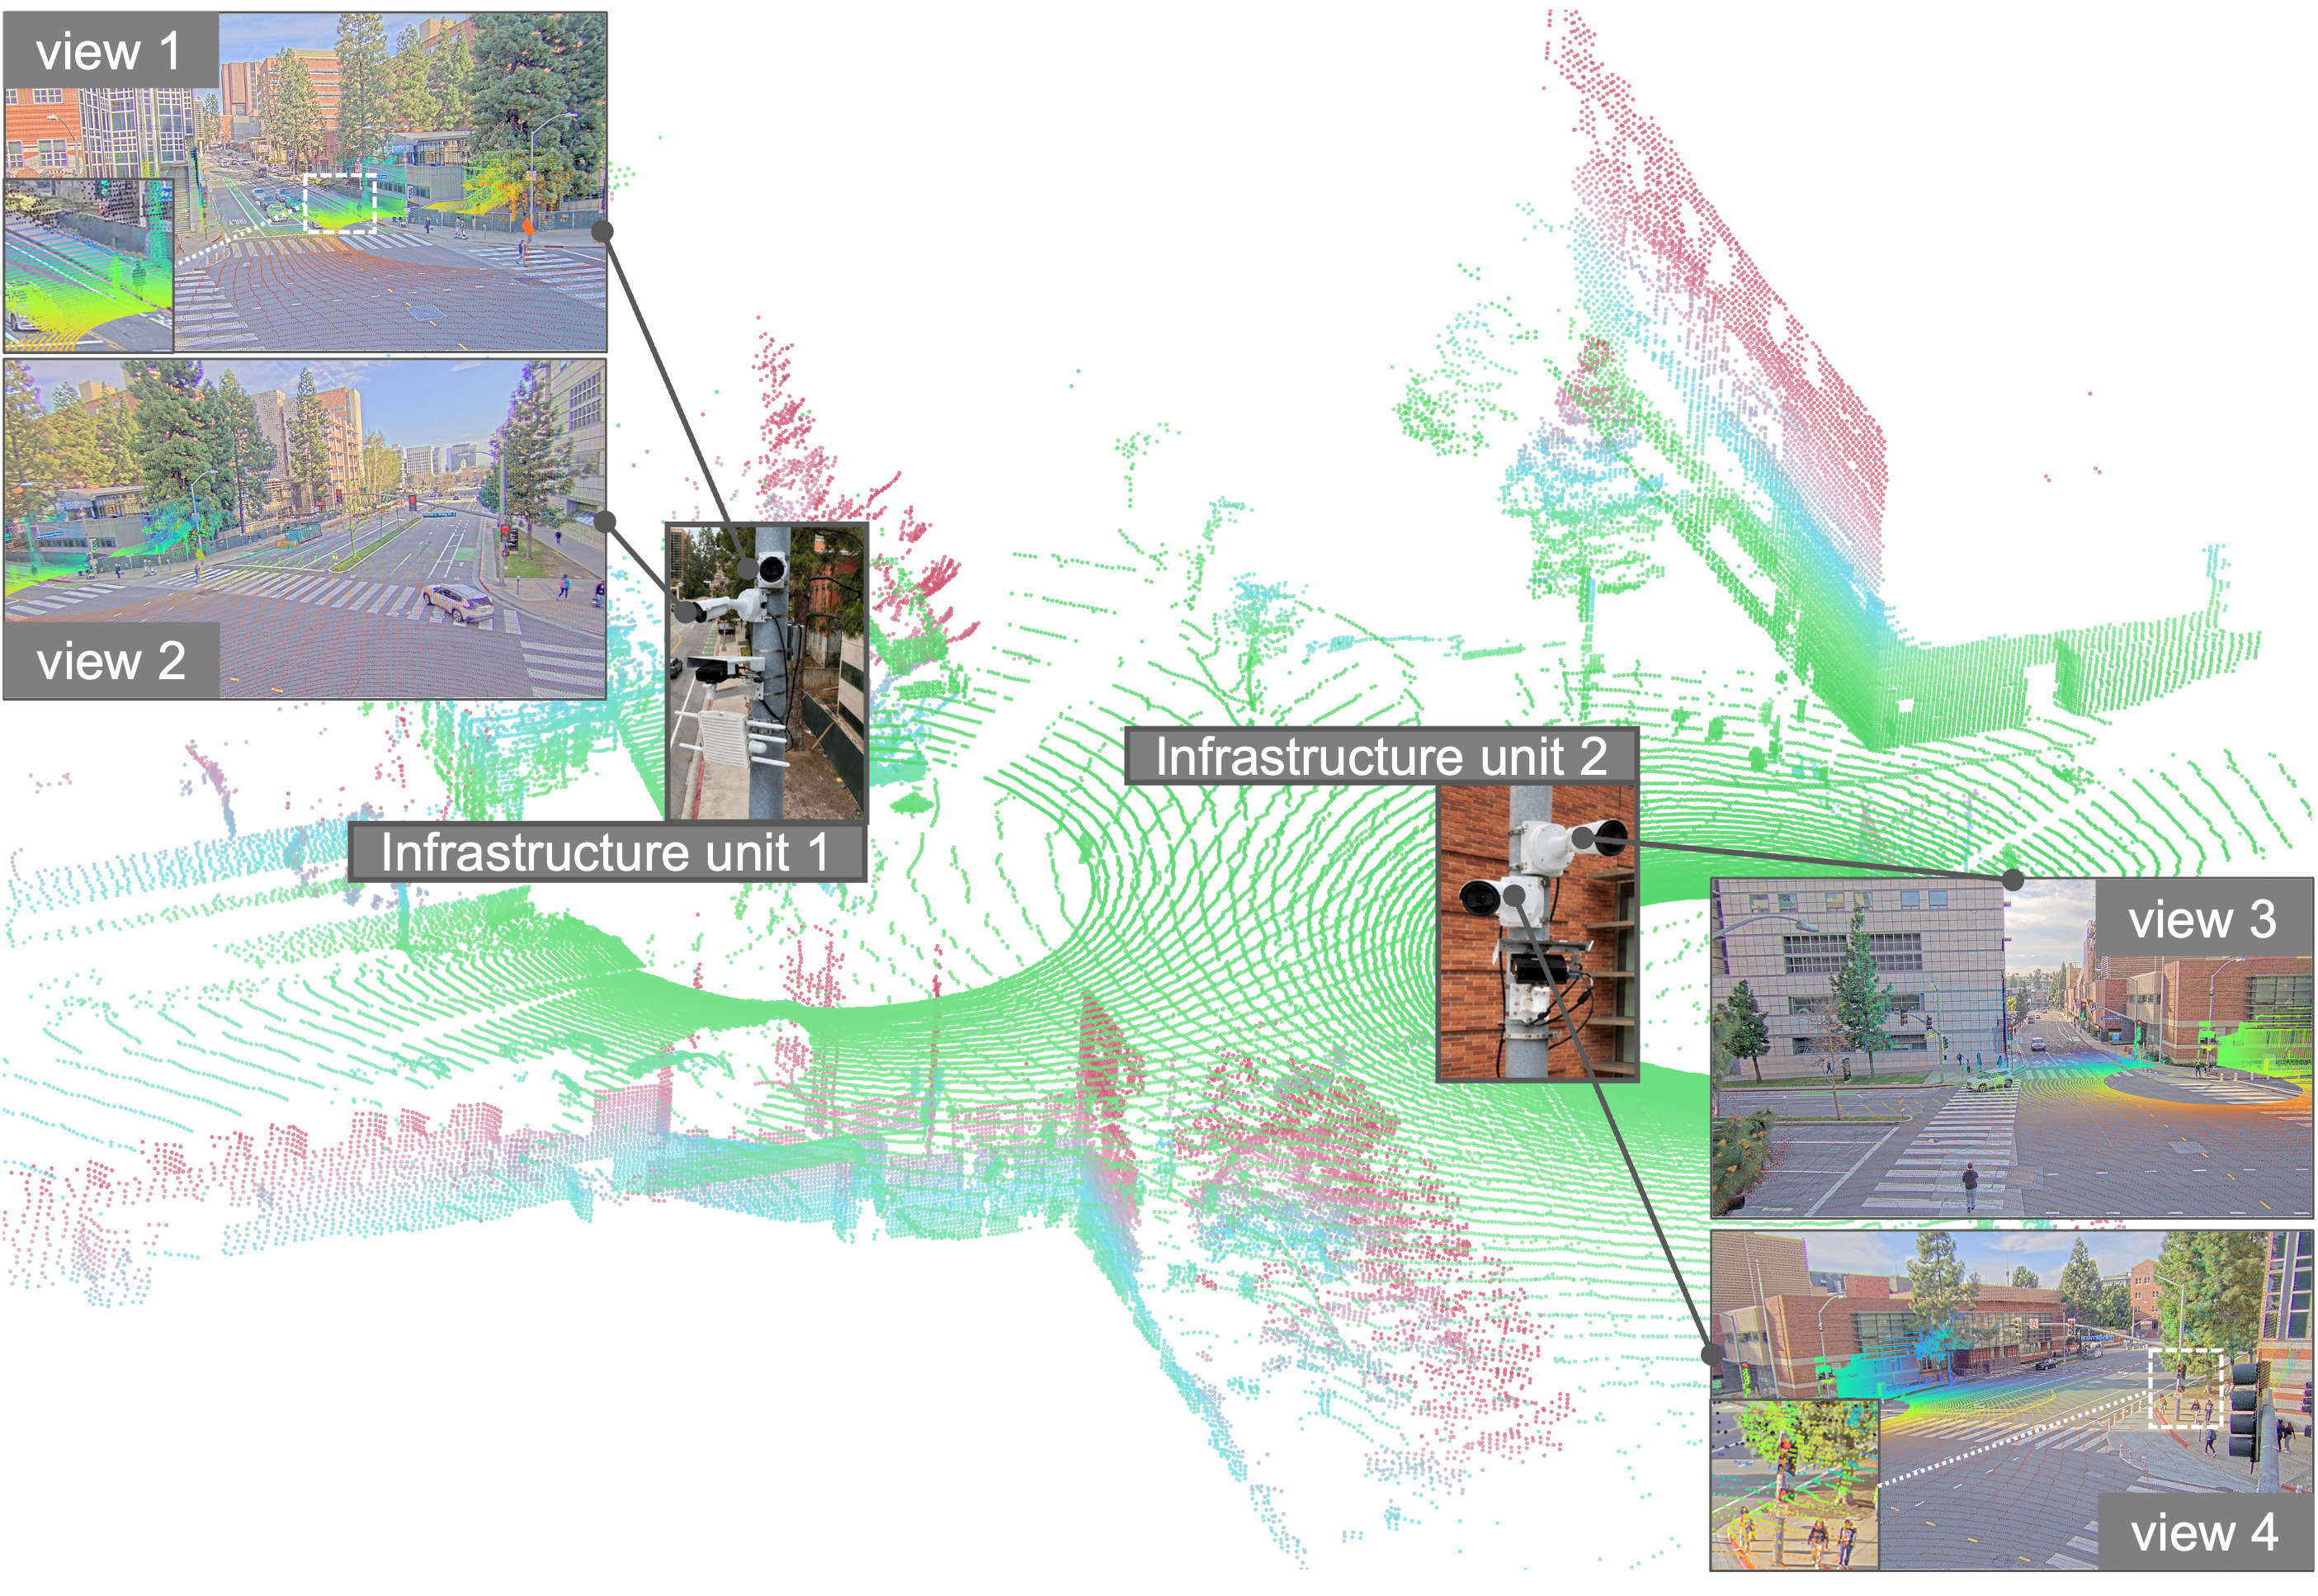
\includegraphics[width=\linewidth]{figures/fig02-sensor-setup.png}
  \caption{\textbf{Infrastructure-side sensor configuration.}
  The roadside platform comprises two fixed infrastructure units, each equipped
  with one LiDAR and two high-resolution cameras under GPS time synchronization.
  Their calibrated streams are organized in a fixed roadside coordinate system
  and support camera-only, LiDAR-only, and multi-modal occupancy prediction.}
  \label{fig:sensor_setup}
\end{figure}


\subsection{Data Source and Sensor Setup}
\label{sec:benchmark_sensor}
\begin{figure*}[!t]
  \centering
  
\includegraphics[width=\textwidth]{figures/fig03-dataset-construction.png}
\caption{\textbf{Overview of the dataset construction pipeline.} We build dense semantic occupancy annotations from two complementary
semantic point-cloud sources: Semantic Dynamic Object Point Clouds constructed from infrastructure-side LiDAR sequences and Semantic Static Background Point
Clouds constructed from vehicle-side LiDAR sequences. The dynamic branch uses manually annotated object tracklets and Tracklet-based Object Alignment to
densify dynamic objects, while the static branch uses Ego-pose Alignment, dynamic-object Removal, and Semantic Annotation to construct persistent
infrastructure layout. Static-dynamic recomposition integrates the two semantic point-cloud sources in the fixed roadside coordinate system, and Occupancy
Labeling converts the recomposed scene into voxel-level semantic occupancy labels.}
\label{fig:dataset_construction}
\end{figure*}

\begin{figure}[!t]
  \centering
  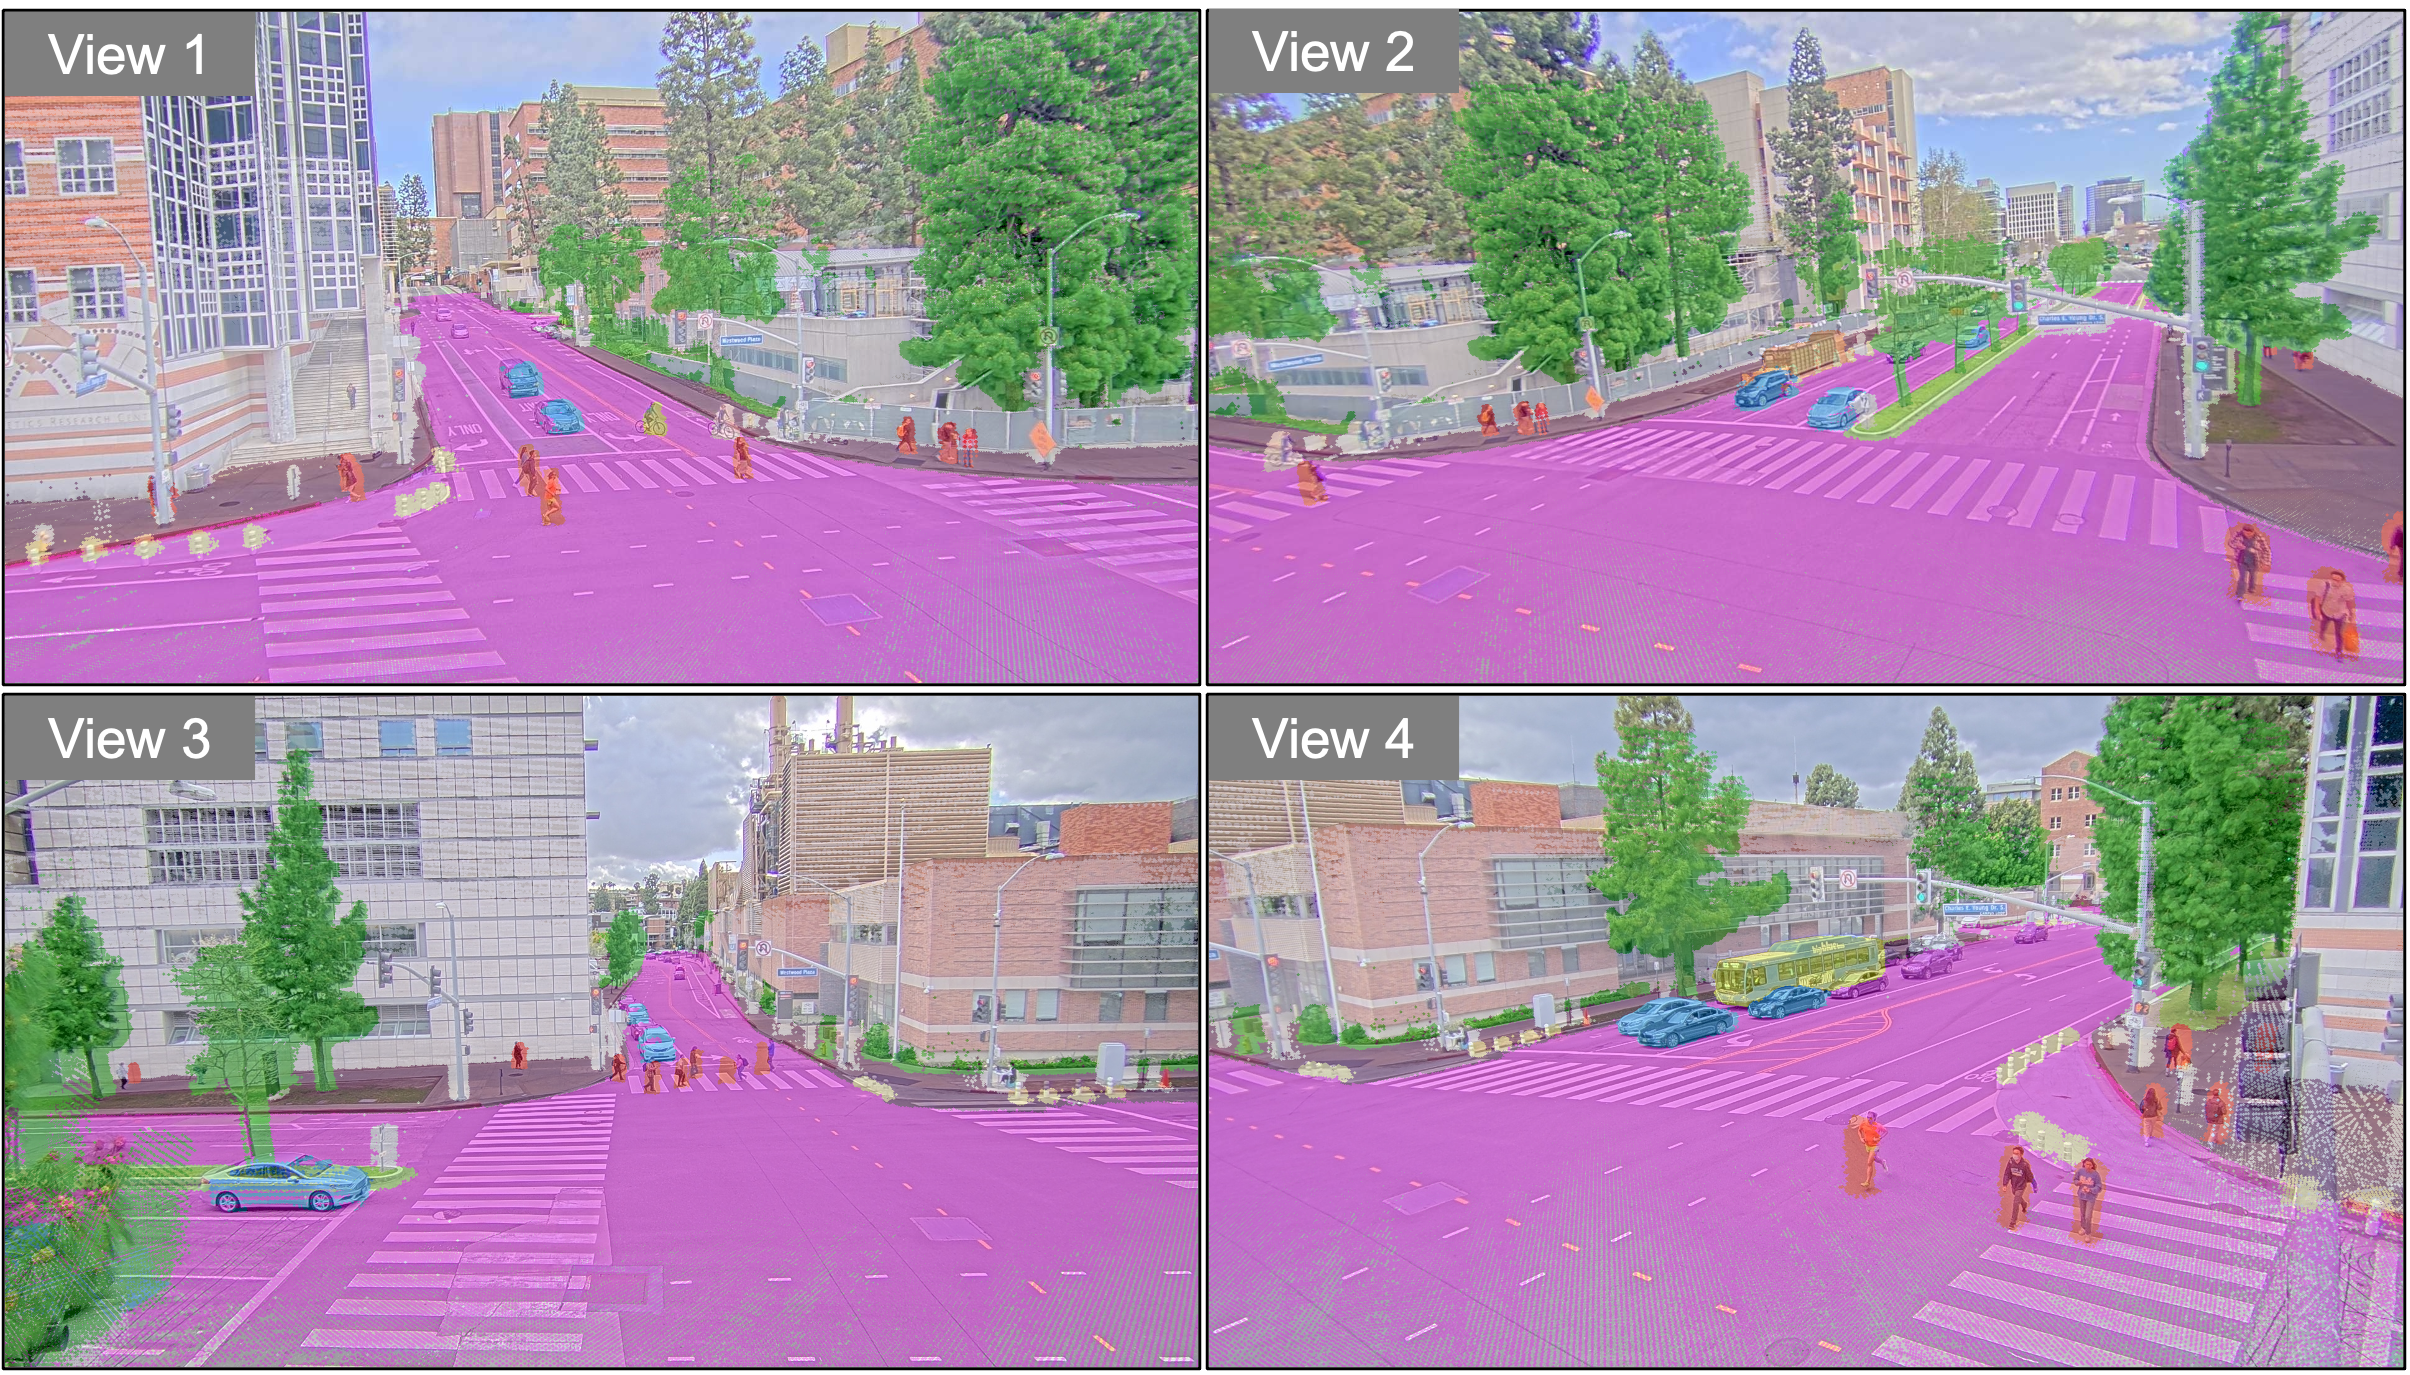
\includegraphics[width=\linewidth]{figures/fig04-2d-3d-quality-check.png}
  \caption{\textbf{Quality check.} The recomposed semantic 3D scene is projected onto the calibrated roadside
  camera views to inspect the alignment between dense point-cloud semantic
  annotations and image observations. Annotators check semantic boundaries,
  object placement, and cross-modal calibration consistency, and manually correct
  any misclassified labels, thereby ensuring the reliability of the
  constructed infrastructure-side occupancy annotations.}
  \label{fig:2d_3d_consistency}
\end{figure}


Our benchmark is built on real multi-modal streams from a fixed roadside
platform of two infrastructure units deployed around a smart intersection and
its adjacent road segments. Each infrastructure unit carries one infrastructure-side LiDAR
(Ouster OS1-128) and two high-resolution Axis cameras ($1920\times1080$) under
GPS time synchronization, yielding four calibrated camera views and two
infrastructure-side LiDAR scans per keyframe over a fixed-view camera--LiDAR
system (Fig.~\ref{fig:sensor_setup}). These streams are provided by
V2X-Real~\cite{V2XReal}, which we
reorganize from the original object-level cooperative 3D detection setting into a
benchmark for dense semantic occupancy prediction.
Since all sensors are fixed, InfraOcc retains the original calibration and
synchronization to align roadside images, LiDAR point clouds, and occupancy
annotations within one fixed roadside coordinate system, enabling camera-only,
LiDAR-only, and multi-modal evaluation under a shared data split and protocol.
Fig.~\ref{fig:dataset_sample} shows a representative keyframe with the four
roadside camera views together with voxel-level semantic occupancy annotations.

\subsection{Dataset Construction Pipeline}
\label{sec:benchmark_pipeline}

\subsubsection{Pipeline Overview}
Fig.~\ref{fig:dataset_construction} illustrates the annotation construction
pipeline of InfraOcc. Infrastructure-side occupancy annotation faces two key
challenges. First, fixed infrastructure-side LiDAR is limited by viewpoint and
occlusion, making it difficult to fully cover persistent infrastructure such as
roads, buildings, vegetation, and barriers. Second, dynamic objects captured by
a single roadside LiDAR scan are often sparse and incomplete, especially around
object boundaries. To address these challenges, InfraOcc adopts a semantic
point-cloud-based construction strategy that decouples static background
completion from dynamic object reconstruction. The upper branch constructs
Semantic Dynamic Object Point Clouds from infrastructure-side LiDAR sequences,
while the lower branch constructs Semantic Static Background Point Clouds from
vehicle-side LiDAR sequences. These two semantic point-cloud sources are then
integrated by Static-Dynamic Recomp. in the fixed roadside coordinate system
and converted into dense voxel-level semantic occupancy annotations through
Occupancy Labeling. Vehicle-side LiDAR is used only for annotation
construction; the benchmark inputs remain infrastructure-side cameras,
infrastructure-side LiDAR, or their combination according to different
evaluation tracks.

\subsubsection{Semantic Dynamic Object Point Clouds}
The upper branch constructs Semantic Dynamic Object Point Clouds from
infrastructure-side LiDAR sequences. We first obtain manually annotated object
tracklets, where each dynamic object is associated with temporally consistent
3D bounding boxes, a semantic category, and a track identity. Based on these
tracklets, object point clouds belonging to the same dynamic object are cropped
from multiple infrastructure-side LiDAR scans.
To aggregate partial observations of moving objects over time, we perform
Tracklet-based Object Alignment. Specifically, the relative poses of 3D boxes
within the same tracklet are used to estimate a box-guided rigid
transformation, which coarsely aligns object point clouds to the reference
object coordinate system. This step compensates for object motion and avoids
motion ghosting caused by direct accumulation in the global frame. ICP
refinement~\cite{Besl1992ICP} is further applied to reduce local misalignment
caused by tracking jitter, box localization errors, and partial occlusion. The accumulated object
point clouds inherit the semantic category of the corresponding tracklet,
forming denser and semantically consistent dynamic object geometry.

\subsubsection{Semantic Static Background Point Clouds}
The lower branch constructs Semantic Static Background Point Clouds from
vehicle-side LiDAR sequences. Since vehicle-side LiDAR observes the same
infrastructure scene from moving viewpoints, it provides more complete
geometric coverage for persistent static elements, including road surfaces,
sidewalks, vegetation, buildings, and barriers. Multi-frame vehicle-side point
clouds are first registered into the roadside coordinate system through
Ego-pose Alignment. Dynamic object points are then removed to prevent transient
traffic participants from being fused into the static background.
Semantic Annotation is performed on the accumulated static background to assign
semantic labels to persistent infrastructure elements. The resulting Semantic
Static Background Point Clouds provide a dense static scene scaffold for the
subsequent Static-Dynamic Recomp.
\begin{figure*}[!t]
  \centering
  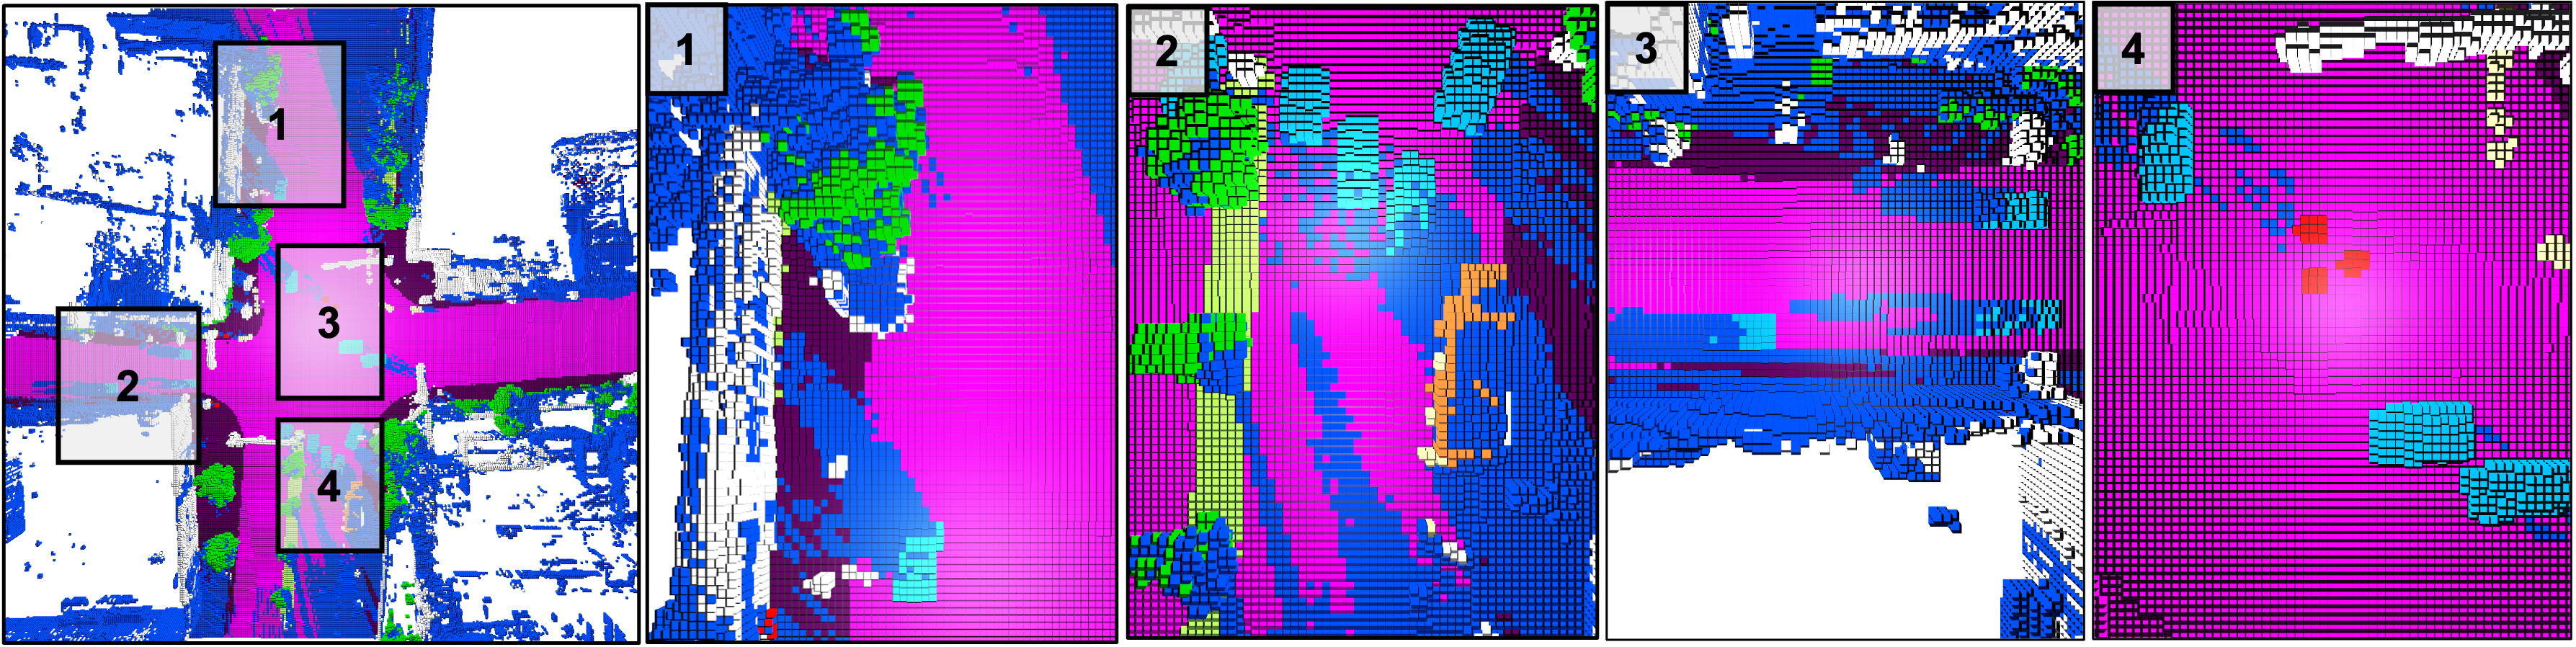
\includegraphics[width=\textwidth]{figures/fig05-camera-mask.png}
  \caption{\textbf{Camera-view visibility masks for occupancy labeling.}
  The voxel grid is projected into calibrated roadside camera views to identify
  image-observable regions in the fixed roadside coordinate system. The left
  panel overlays the visibility masks of four roadside views on the semantic
  occupancy map, while the right panels show enlarged local regions for each
  camera view. These masks describe camera observability and support
  consistency inspection between roadside images and voxel-level semantic
  occupancy annotations.}
  \label{fig:camera_mask}
\end{figure*}


\subsubsection{Static-Dynamic Recomposition}
After constructing Semantic Dynamic Object Point Clouds and Semantic Static
Background Point Clouds, we recompose them into keyframe-level semantic scenes
in the fixed roadside coordinate system.

\noindent\textbf{Static-Dynamic Recomposition.}
For each keyframe, the Semantic Static Background Point Clouds serve as a
persistent scene scaffold. Dynamic object point clouds are transformed into the
roadside coordinate system according to their tracklet poses at the current
timestamp and inserted into the static background. This produces a semantic 3D
scene that preserves both stable infrastructure layout and keyframe-specific
traffic participants, while avoiding motion artifacts caused by directly
accumulating moving objects.

\noindent\textbf{Image-guided Verification.}
We further project the recomposed semantic scene onto calibrated roadside
camera views to inspect its consistency with image observations. As shown in
Fig.~\ref{fig:2d_3d_consistency}, this verification checks semantic boundaries,
dynamic object locations, and cross-modal calibration consistency before
voxel-level occupancy labeling.


\subsubsection{Occupancy Labeling}
After static-dynamic recomposition, each keyframe is represented as a semantic
3D scene containing both persistent infrastructure layout and keyframe-specific
dynamic objects. Occupancy Labeling converts this recomposed scene into
voxel-level semantic occupancy ground truth. Similar to Occ3D~\cite{Occ3D}, we
distinguish three voxel states: occupied, free, and unobserved, so that empty
space and occluded regions are not confused.

\noindent\textbf{Semantic Occupancy GT.}
We first discretize the recomposed semantic point clouds into the predefined
voxel grid. Voxels containing semantic points are labeled as occupied and
assigned the corresponding semantic category. Static background points provide
labels for persistent infrastructure elements, while dynamic object points
provide labels for traffic participants at the current keyframe. In this way,
static layout and dynamic objects are represented in the same fixed roadside
coordinate system.

\noindent\textbf{Visibility Reasoning.}
Voxels without semantic points are further processed by visibility reasoning.
We trace infrastructure-side LiDAR rays from the sensor origin to observed
surfaces. Voxels traversed before the first occupied surface are labeled as
free space, while voxels behind observed surfaces or outside valid sensor rays
are treated as unobserved and ignored. This prevents occluded regions behind
buildings, vegetation, or vehicles from being incorrectly labeled as free.
We further compute camera-view visibility masks by projecting voxel centers
into calibrated roadside cameras. A voxel is regarded as camera-visible if its
projected center lies inside the image boundary with positive depth.
Fig.~\ref{fig:camera_mask} visualizes the resulting masks, which characterize
the image-observable regions of different roadside cameras and support
consistency inspection between roadside images and voxel-level semantic labels.


\subsection{Dataset Statistics}
\label{sec:benchmark_statistics}

\subsubsection{Scale and Annotation Coverage}
InfraOcc contains 290 temporally continuous roadside sequences (215 for
training and 75 for evaluation), each spanning roughly 10--24 seconds. Raw
streams are recorded at 10 Hz, while dense semantic occupancy is annotated on
2 Hz keyframes (every fifth raw frame), preserving short-term traffic evolution
while keeping the benchmark focused on keyframe-level prediction. Each annotated
keyframe provides four calibrated roadside camera views, two infrastructure-side
LiDAR scans, and one dense voxel-level occupancy annotation over the range
$[-64,64]\!\times\![-64,64]\!\times\![-4.8,1.6]$~m at a $0.4$~m voxel size, i.e.,
a $320\times320\times16$ grid; its label space comprises the occupied semantic
classes and a free-space class, supporting both semantic and category-agnostic
geometry evaluation.


\begin{figure}[t]
  \centering
  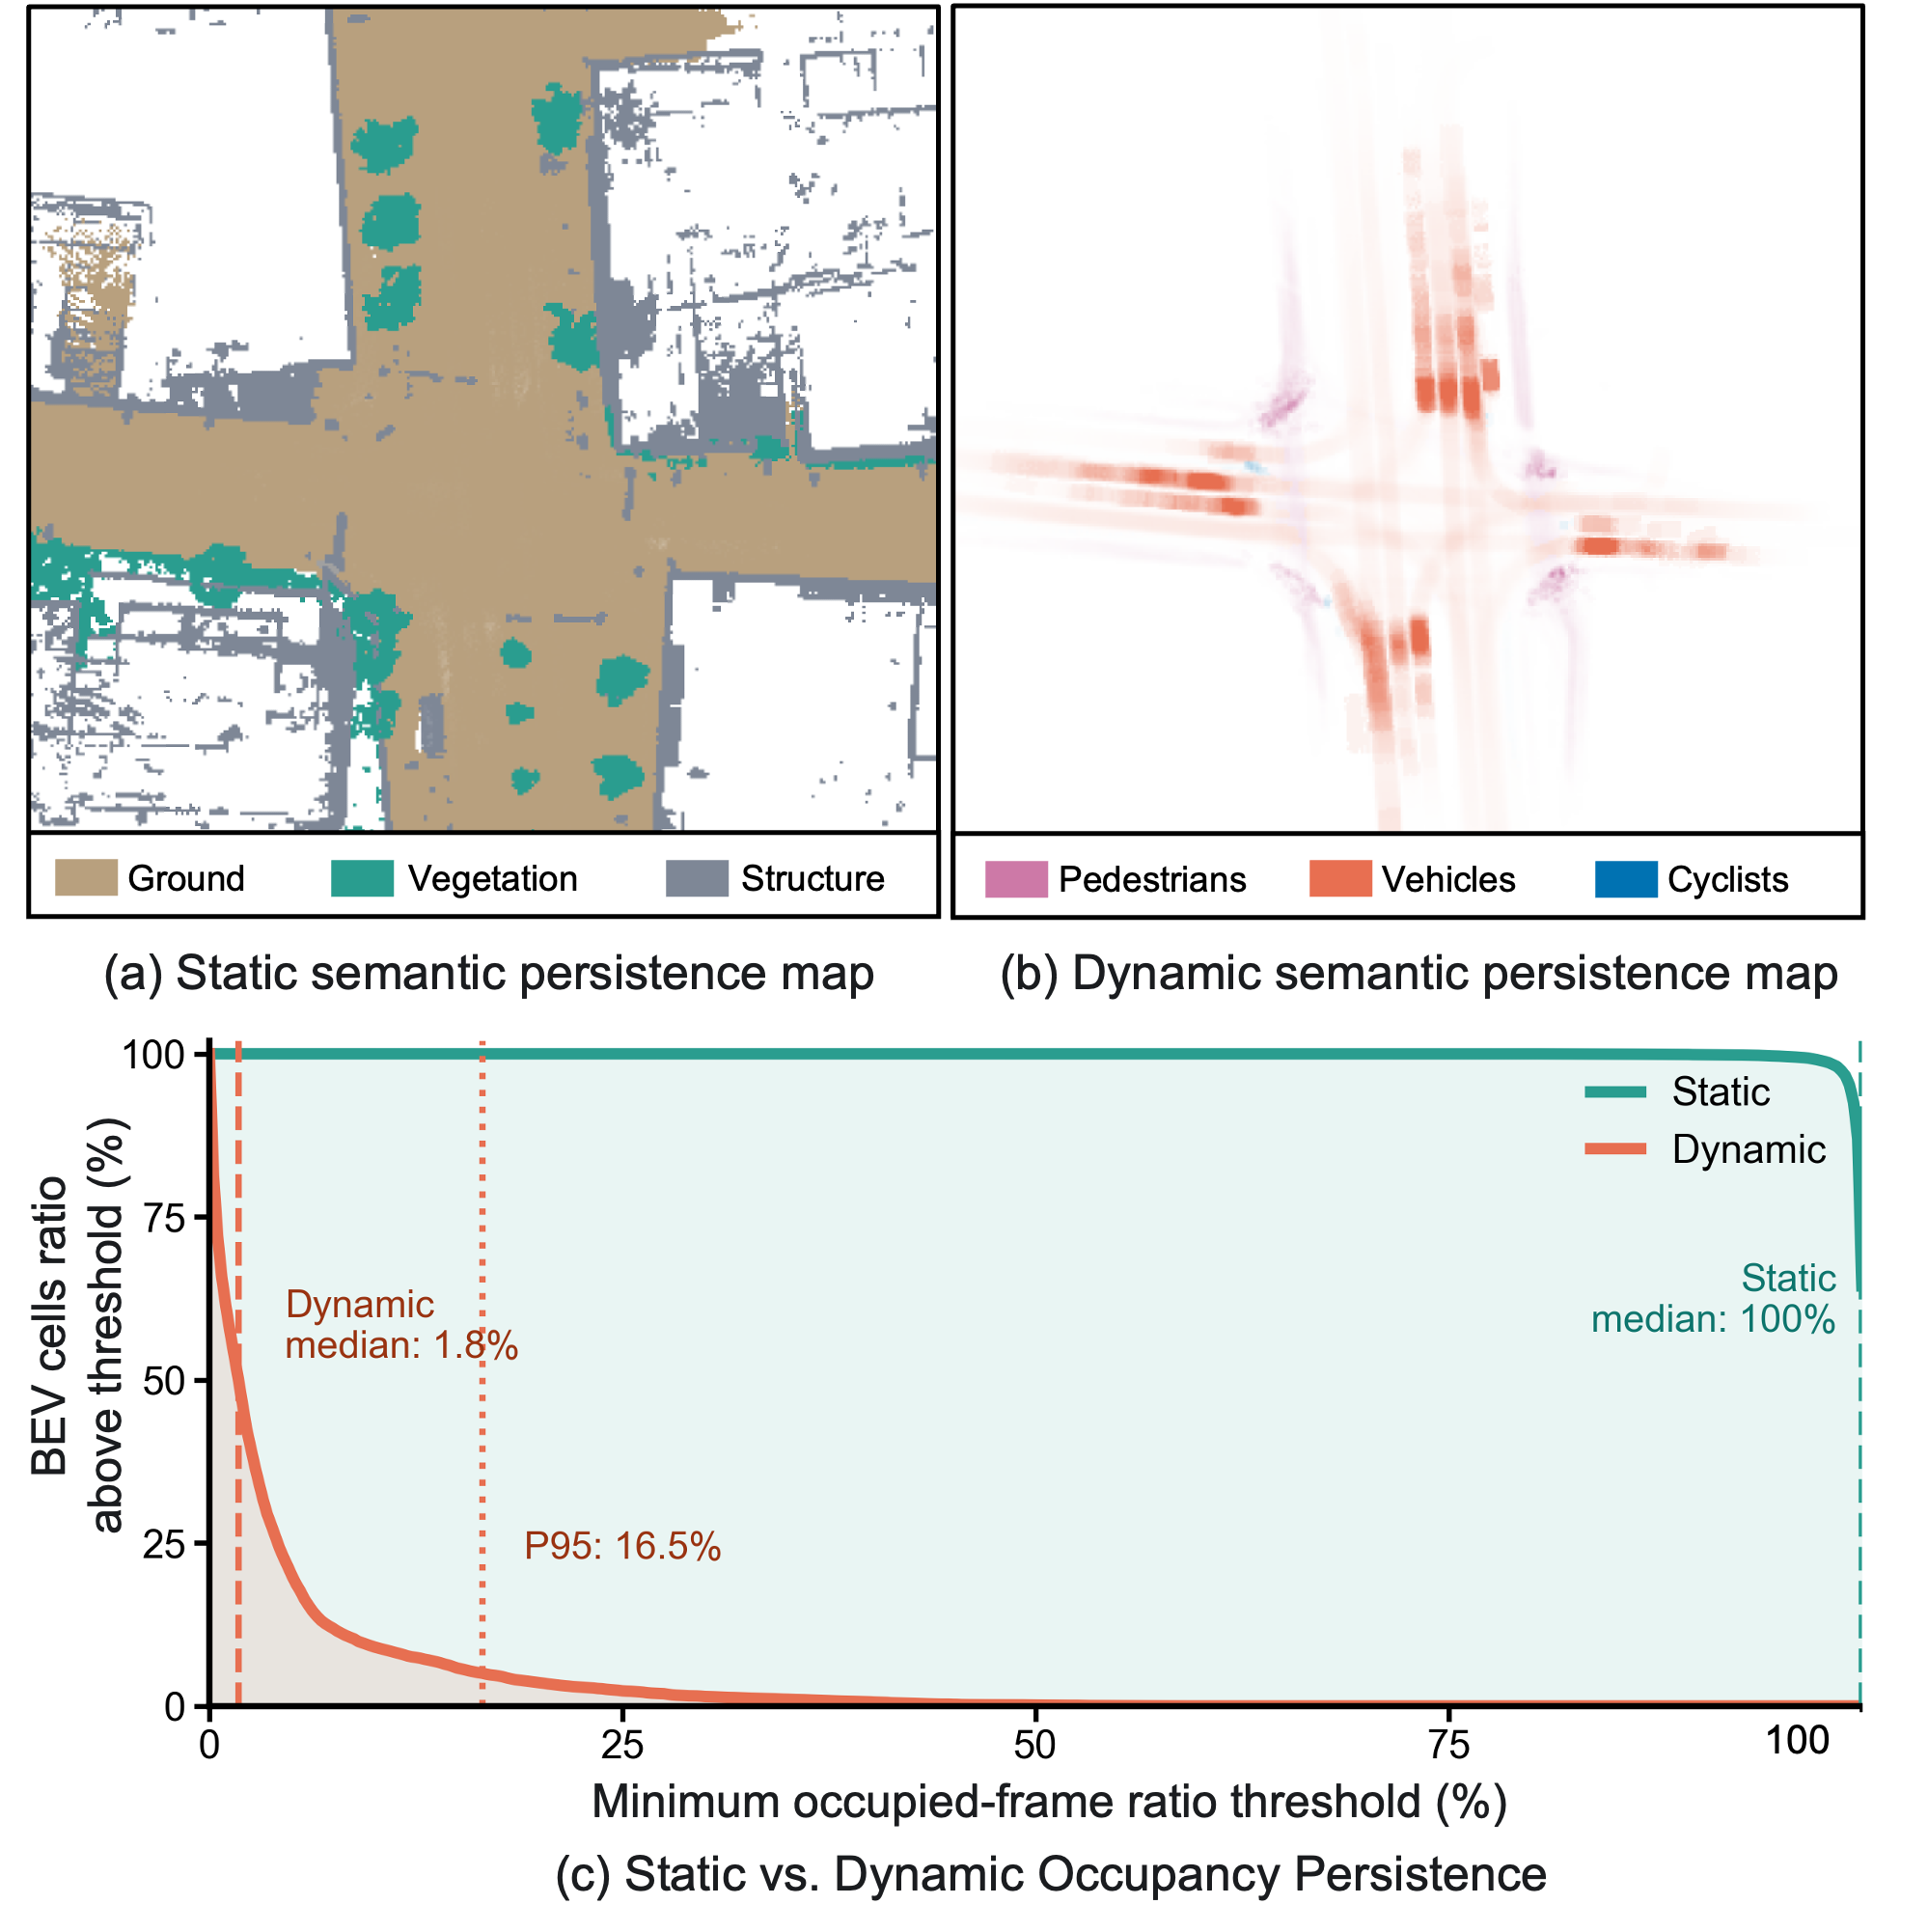
\includegraphics[width=\linewidth]{figures/fig06-temporal-statistics.png}
  \caption{\textbf{Static-dynamic occupancy persistence statistics.}
(a) Static semantic persistence map in the fixed infrastructure coordinate
system. Colors denote dominant coarse static groups, and color intensity
indicates the occupied-frame ratio of each BEV cell. (b) Dynamic semantic
transience map computed in the same BEV space, where dynamic occupancy mainly
appears along lanes, crosswalks, and typical traffic trajectories. (c)
Occupancy persistence curve. The horizontal axis denotes the minimum
occupied-frame ratio threshold, and the vertical axis denotes the BEV cells ratio
retained above the threshold. % Static regions remain highly persistent, whereas dynamic regions are sparse and transient.
}
\label{fig:spatiotemporal_semantic_statistics}
\end{figure}

\begin{figure}[h!t]
  \centering
  
\includegraphics[width=\linewidth]{figures/fig07-class-distribution.png}
  \caption{\textbf{Semantic class distribution.}
The top strip summarizes occupied voxels by semantic group, while the lower
panel reports class-wise voxel occupancy ratios over evaluated occupied
classes. The vertical axis is
shown in log scale for readability. The distribution shows that static
infrastructure dominates the occupied semantic space, whereas dynamic traffic
participants form a sparse long-tailed subset.}
  \label{fig:semantic_class_distribution}
\end{figure}



\subsubsection{Static-Dynamic Temporal Asymmetry}
Beyond dataset scale, InfraOcc exhibits a distinctive static-dynamic temporal
asymmetry caused by fixed infrastructure-side observation. Roadside sensors
observe the same traffic space over time, so persistent infrastructure elements
repeatedly appear in consistent spatial regions. In contrast, dynamic traffic
participants occupy local regions only for short periods and mainly appear
along lanes, crosswalks, and typical motion trajectories.
To quantify this property, we project voxel-level semantic labels along the
height dimension into BEV space and compute the occupied-frame ratio for each
BEV cell, defined as the fraction of frames in which the cell is occupied by a
static or dynamic semantic group. For visualization, semantic labels are
regrouped into coarse categories, while benchmark evaluation still follows the
full semantic label space.
Fig.~\ref{fig:spatiotemporal_semantic_statistics} summarizes the resulting
spatio-temporal occupancy statistics under the fixed infrastructure coordinate
system. In Fig.~\ref{fig:spatiotemporal_semantic_statistics}(a), each BEV cell
is colored by its dominant coarse static group over time, and the color
intensity encodes the occupied-frame ratio. The resulting map shows that
ground, vegetation, and structural regions form spatially continuous and
high-persistence layouts, reflecting the stable infrastructure scaffold
observed by fixed roadside sensors. Fig.~\ref{fig:spatiotemporal_semantic_statistics}(b)
is computed in the same BEV space but only over dynamic groups. Compared with
the static map, dynamic occupancy appears as sparse and low-intensity traces
along lanes, crosswalks, and typical traffic trajectories, indicating that
dynamic objects repeatedly pass through certain regions but rarely occupy the
same BEV cell for long periods. 
Fig.~\ref{fig:spatiotemporal_semantic_statistics}(c) further quantifies this
contrast using an occupancy persistence curve. The horizontal axis denotes the
minimum occupied-frame ratio threshold, and the vertical axis reports the ratio
of BEV cells retained above that threshold. Static cells remain almost fully
retained across most thresholds, with a median occupied-frame ratio of 100\%.
In contrast, dynamic cells quickly vanish as the threshold increases, with a
median ratio of only 1.4\% and a 95th percentile of 15.7\%. These observations
show that infrastructure-side occupancy has a clear persistent-static versus
transient-dynamic structure: static layout forms a stable spatial scaffold,
whereas dynamic traffic participants provide sparse, short-lived local evidence.

\subsubsection{Semantic Long-tail Distribution}
In addition to temporal asymmetry, InfraOcc also exhibits a pronounced semantic
frequency imbalance. Fig.~\ref{fig:semantic_class_distribution} reports the
class-wise voxel occupancy ratio over evaluated occupied classes, excluding
free space and ignored categories. Static infrastructure categories account for
97.3\% of occupied voxels, whereas dynamic traffic participants account for
only 2.7\%.
The distribution is highly concentrated within static classes: driveable
surface and manmade structures dominate the occupied space, followed by
sidewalk and vegetation. Dynamic classes form a long-tailed subset, where cars
are the most frequent dynamic category, while trucks, motorcycles, and bicycles
are substantially sparser. This semantic long-tail, together with the temporal
asymmetry above, suggests that infrastructure-side occupancy prediction requires
not only overall semantic accuracy, but also group-wise diagnosis of persistent
static layout and sparse dynamic objects.

\subsection{Evaluation Protocol}
\label{sec:benchmark_eval}

InfraOcc evaluates camera-only, LiDAR-only, and multi-modal occupancy under
a unified protocol: all tracks share the same data split, label space,
calibration, and fixed roadside coordinate system, and are evaluated over the
full $320\times320\times16$ grid (Sec.~\ref{sec:benchmark_statistics}) rather
than only sensor-visible regions. Following common occupancy
benchmarks~\cite{OpenOccupancy,Occ3D}, the primary metric is the mean IoU over
valid occupied classes,
\begin{equation}
  \mathrm{mIoU}_{\mathrm{all}}
  =
  \frac{1}{|\mathcal{C}_{\mathrm{eval}}|}
  \sum_{c\in\mathcal{C}_{\mathrm{eval}}}
  \frac{\mathrm{TP}_{c}}{\mathrm{TP}_{c}+\mathrm{FP}_{c}+\mathrm{FN}_{c}},
\end{equation}
where $\mathcal{C}_{\mathrm{eval}}$ excludes free space and the ignored
categories (construction vehicle, trailer, and other flat; omitted due to
sparsity or ambiguous boundaries), and free space is reported separately as
\textit{Free} IoU. To diagnose the static--dynamic asymmetry, we additionally
report gIoU (the IoU of all non-free classes merged into a single occupied
group) and the group-wise mIoU$_{\mathrm{dyn}}$ / mIoU$_{\mathrm{sta}}$, i.e.,
mIoU restricted to the dynamic classes (bicycle, bus, car, motorcycle,
pedestrian, truck) and the static classes (others, barrier, traffic cone,
driveable surface, sidewalk, terrain, manmade, vegetation), respectively.
Together with per-class IoU, these metrics evaluate geometry, static layout,
dynamic objects, and free space across modalities.
